\chapter{Introduction}\label{ch1}


%Introduction+conclusion are shorter chapters

%Introduction
%Hypothesis
%research questions
%context
%Summary of the contributions
%Good to introduce gently but research questions can be fine
%Doesn't have to be accessible to the man on the street, need computer science background, vector spaces are included in that, so are decision trees and neural networks, if it's borderline reference background

%%Conclusion revisits research questions, provides the answer not just a summary

\section{Introduction}

%%%%% INTRODUCTION

% There is a lot of data, and a lot of good applications of machine-learning using that data

Applications that enable user-generated content e.g.\ Wikipedia, Social Media sites (Facebook, Twitter), Product and movie review sites (IMDB, Rotten Tomatoes, Amazon) and content-aggregation sites (Reddit, Tumblr) have resulted in widely available unstructured text data. This increased availability of text data has resulted in machine-learning models achieving state-of-the-art results on  a variety of problems e.g.\ machine translation \cite{Wu}, question answering \cite{Fisch2016}, or text classification. There are many applications of text classification tasks, e.g.\  using text data to identify if social media posts or product reviews have a positive or negative sentiment about a product \cite{Burel2018},  identifying social media posts  that are useful to crisis responders during crises \cite{Burel2018}, or  predicting depression in social media users \cite{Aldarwish2017}. 

% Machine-learning models are essentially trying to get features that are meaningful in the domain and can so predict something specific

Historically  to achieve strong results in Natural Language Processing tasks, expert knowledge was used, for instance in the form of a knowledge base \cite{Lewis1993}. However, as the volume of available text data has risen,  machine-learning techniques that leverage large amounts of unstructured data are  state-of-the-art in many fields\footnote{https://github.com/sebastianruder/NLP-progress}. To achieve such results, a critical question is how to process the unstructured data so that it can be used by machine-learning models. Ideally, it  can be processed computationally and as much information as possible is encoded. In the case of this thesis, representations of text documents in a variety of domains are used. One example of the data used is the domain of movie reviews, where each movie is represented by a document that is a concatenation of all of its IMDB reviews.    One simple and common method to pre-process unstructured text documents is to represent them by the frequency of words  in their documents. This  representation  is called a "Bag-of-words", as word context is discarded. %However, word context,  An example where word context is important would be when the sentiment  of an Amazon product review would be classified. If a user was sarcastic in their review, For example if a review of a calendar with a printing error was "This product is so supremely excellent that it is totally blank", then the the classifier would perform better if the  context of the words was included in the representation, so it could distinguish sarcasm.  % resulted in a variety of ways to take advantage of it, 

% Representations are a fundamental part of good machine-learning. 

%Similar to how it would not be possible for a human to solve a problem without a good understanding of the subject area, the first step of solving a problem with  machine-learning  is to obtain a suitable  representation of the data. If this  representation is not good, then no matter what steps are taken to try and solve the problem then they will not yield good results. Representations are typically composed of features, where each feature is some specific property of the domain that can be used to represent an entity. For example, when classifying if a person should be given a loan, people entities are represented by features of how much they earn, if they are a small business owner, and if they have a family. 

% But what is a good representation. How do you get a good representation. What are the advantages/disadvantages? Improtance of unsupervised reprsentations

%One way to obtain a representation of the data that results in strong performance is feature engineering [cite], integrating encoded domain knowledge [cite], or using experts to validate the features [cite].  Manually hand-crafting or improving features takes time and knowledge that is not available for many domains, and so methods have been developed to learn features from data without the need of hand-labelling or encoding expert knowledge [cite].

% What are vector spaces? Why are they used? Why are they important and what are they a part of? What are their disadvantages?

Bag-of-words are limited in the amount of information they represent. Ideally, a representation  derived from a domain  encodes as much information  as possible  while utilising a large amount of data, and is flexible in the information it can represent. This is typically done by inducing a low-dimensional vector space representation. Vector spaces of documents, or 'semantic spaces' represent  semantic relationships between documents in the domain  spatially. For example, in a domain of movie reviews, horror movies would be spatially close to each other, and romance movies would be spatially distant from horror movies. The problem with these semantic spaces, especially those learned from neural networks, is that despite the fact that these representations clearly capture meaning in a non-trivial way, it is not clear how meaningful features can be extracted from such representations. Specifically, the dimensions of these vector space embeddings do not typically have any particular meaning.
%For example, word-vectors \cite{Pennington2014} \cite{Mikolov2013} learned from a large corpora like Wikipedia encode the meaning of words spatially by leveraging their context across millions of documents, resulting in e.g. spatial analogical relationships, where vec(man) corresponds to the vector space representation of the word "man", vec(man) - vec(king) $\approx$ vec(woman) - vec(queen). 




% What is disentanglement? How does it relate to machine-learning feature Interpretability?  Why is it important?

 % and overlapping regions occur that correspond to properties of the domain (e.g. "tasty", "acidic", "bitter", "exotic"). Below, an example is shown of such a vector space.
 
%

In neural representation learning, representations that have separated the 'factors of variation' are referred to as "disentangled" representations \cite{Bengio2012}. For example, a disentangled representation in a domain of images of handwritten digits  has a  dimension for the style of the digit  and separate dimensions for what digit is written   \cite{Chen2016}. In a text domain, disentangled representations separate dimensions for the sentiment of the text and dimensions for their content    \cite{John2019}, and in the medical domain a representation is separated into key medical features that doctors use to formulate clinical questions \cite{Banner}. Disentanglement has many benefits, such as transforming the representation of an entities feature like sentiment while leaving the content intact \cite{Larsson2017}, providing an inductive bias in machine-learning models, and potentially leading to better generalization, increasing the potential for transfer learning, and resulting in more efficient unsupervised learning  \cite{Banner}  \cite{Paige2016}.   

Disentangled representations  are linked to the objective of interpretability. As machine-learning has extended into  real-world domains like medicine and policing,  the legality and risk of implementing systems that do not have easily understood features (e.g. vector spaces) has resulted in concerns of safety (providing the wrong decision in a high-risk domain), fairness (using properties like  the race of a person to e.g. deny a loan), and transparency (being able to know what the model is doing and improve it) have not been accommodated. The EU have introduced a legal "Right to explanation", requiring that machine-learning models must be able to explain why they have made a decision about a person. However,  disentangled representations do not typically claim that they will be interpretable in the sense  they explain their behaviour to human users. Instead, the focus is that the key factors of the domain are separated into dimensions of the representation,  and this is validated by investigating how these dimensions behave. This distinction is primarily one of application. Disentangled feature representations may indeed be interpretable, but they are typically used for functional purposes rather than explanatory ones.

%Such publica- tions constitute the evidence drawn upon to sup- port evidence-based medicine (EBM), in which one formulates precise clinical questions with re- spect to the Populations, Interventions, Compara- tors and Outcomes (PICO elements) of interest (Sackett et al., 1996).1


%There are multiple advantages to advancing this area of research. Neural networks have been used to disentangle style and content in a latent space to transfer style \cite{John2019}, disentangle key aspects of clinical questions in a medical text domain (Populations, Interventions, Comparators and Outcomes)  for the sake of efficient model transfer and interpretability \cite{Banner}, transform the sentiment of text while leaving the content intact \cite{Larsson2017}, 

%Variational auto-encoders by enforcing independence \cite{Hu2017}  disentangle key aspects in multiple  domains (images and text) by enforcing statistical independence \cite{Paige2016}.

%Firstly, there are not many approaches that can induce disentangled representations in the domain of text, as 

%"Thus far in NLP, learned distributed represen-
%tations have, with few exceptions (Ruder et al., 2016; He et al., 2017; Zhang et al., 2017), been en- tangled: they indiscriminately encode all aspects of texts. Rather than representing text via a mono- lithic vector, we propose to estimate multiple em- beddings that capture complementary aspects of texts, drawing inspiration from the ML in vision community (Whitney, 2016; Veit et al., 2017a)" \cite{Banner}

%Benefits of disentanglement: Knowing if the model will generalize, transfer learning, more effiicent training when supervised objectivers are not aviavlalb,e  

 %Different from other vector space models, however, a conceptual space is typically composed of several vector spaces, each of which intuitively models a single facet from the given domain. For example, a conceptual space of fruit could be composed of vector spaces modelling color, shape, taste, price, size and weight.

%A conceptual space is   They represent entities (e.g. in a conceptual space of fruit, entities are "orange" "apple" "watermelon") as points in a vector space  where  dimensions  correspond to primitive features of the domain (e.g.\ color, shape, taste in a conceptual space of fruit). As an example from a domain of text documents, in a domain of movie reviews, entities would be movies. 

This thesis follows work by Derrac \cite{Derrac2015}  that assumes that  spatial relationships in a document embedding of entities can be derived to obtain semantic features. Essentially, vector space embeddings can be re-organized into semantic features that correspond to spatial relationships in the original vector space embedding. Their method ranks documents on features, for example in a domain of IMDB movie reviews, movies would be ranked on how "Comedic" they are. The process to obtain these rankings is as follows: First, linear classifiers (e.g. linear Support Vector Machines) are used with the vector-space as input, and a hyper-plane is found that separates entities  where the word occurs at least once and those where the word did not occur. To see an example in 2-dimensional space, see Figure \ref{ch1:introhyp}. Second, the orthogonal direction from that hyper-plane is taken, resulting in a direction that starts  far from the hyper-plane on the negative side (those that least have the feature) and ends far from the hyper-plane on the positive side (those that most have the feature). Finally, entities are ranked on that direction using the dot-product and that ranking is used as a feature. An accompanying visual to explain directions and rankings is shown in Figure \ref{ch1:introhyp}.  %derived from vector directions in the representation that go from entities that least have a property (e.g. movies that are the least "Funny") to those that  have it the most. 

\begin{figure}[t]
	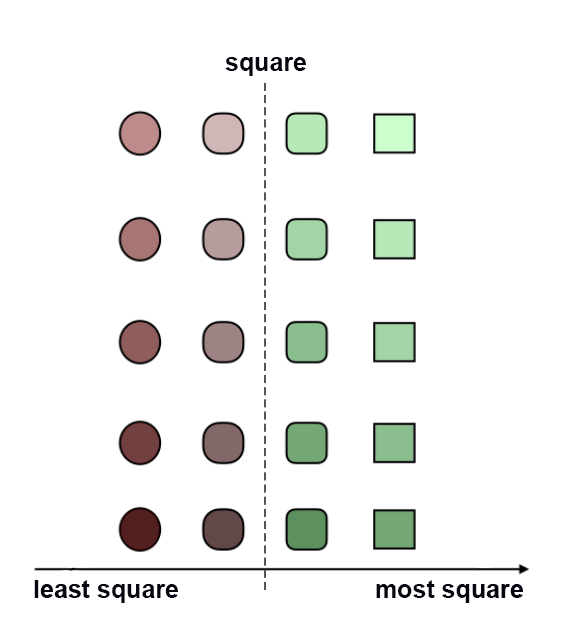
\includegraphics[width=250px]{images/Toyhyperplane1Direction.png}
	\centering
	\caption{An example of a hyper-plane in a toy domain of shapes. The hyper-plane for the word square is the dotted line. Green shapes are positive examples and red shapes are negative examples. Those closest to the hyper-plane are less square than those further away. The arrow along the bottom of the figure is the direction, and rankings on that direction can be derived from how far along the shapes are on that direction}\label{ch1:introhyp}
\end{figure}


Previously, disentanglement has required particular  neural network architectures and learning methods, typically by learning a representation with a requirement that features must be independent from each other \cite{Banner}  \cite{Paige2016}. The aim of this thesis is to study and develop unsupervised methods for learning disentangled representations as a post-processing step on existing vector space embeddings, following the work by Derrac \cite{Derrac2015}. In particular, the method from Derrac \cite{Derrac2015} is expanded on such that disentangled representations derived by the method from vector space embeddings are composed of semantic features. When classifying the sentiment of an Amazon product review, an example of good semantic features in a  disentangled representation are features that directly relate to sentiment, e.g. ranking reviews on how "safe", "reliable", "good", "worthwhile" the product is. 


%For this method, disentangled features are labelled, and e.g. in a domain of movie review documents where movies are represented by a concatenation of all their reviews, words like "Scary" or "Comedy" would be properties that movies are ranked on. However, this thesis does not attempt to validate the interpretability of these associated words or clusters of words. Rather, the focus is on validating that these features are indeed disentangled by testing them on tasks where dense but disentangled features (where the features must correspond to an important domain property and also  encode a large amount of information) would perform well. 

%Fundamentally, both of these views seek to find the essential components that determine why all entities vary in the domain, and use them as features. In the case of text processing which we investigate in this work, the factors of variation found correspond to clusters of words that represent properties in the domain. The representation is considered disentangled if the features obtained are interpretable and  predictive when used in key domain tasks.





 %This, among others, has catapulted machine-learning into the limelight of interpretability, and the result has been swathes of research in both explaining black-box machine-learning models and making machine-learning models interpretable, for good reason.

% What are methods to obtain interpretable features? What are methods to disentangle features?

%Methods that obtain interpretable representations include topic modelling with e.g. Latent Dirchlet Allocation (LDA), Negative Matrix Factorization (NMF), among others. 

%What is the specific case that we want disentangled features for that justify the method?  Explain exactly what the disentangled feature representation is

% What does this thesis do to address that specific case?

% that by separating the key properties of the domain into features,
%The advantage of disentangled representations in this regard is that if the properties of disentangled representations are indeed distinct important concepts in the domain, then that is a first step towards a representation where each feature can be understood by humans. From that representation,  effective machine-learning models can be learned that can explain themselves using these features. However, 

%This thesis offers a new approach for obtaining good disentangled representations, crucially being unsupervised, applied in the text domain, and used as a post-processing step on existing vector space representations. From these features, standard requirements like clustering, classification using simple classifiers, and understanding domains can be achieved, while using the information stored in a representation learned using a large volume of data from e.g. a complicated neural network architecture. 

%ssssssssssssssHowever, these methods lack the flexibility and broad usage of vector spaces, which are applied in a variety of tasks and are a primary component of neural networks, a method that achieves state-of-the-art in many tasks using text data and in other domains.  This thesis follows work by \cite{Derrac2015} who introduced a method to re-organize text document representations that encode semantic relationships such that these spatial relationships are used as features. Essentially, this work investigates unsupervised methods of post-processing vector spaces to re-organize them into disentangled feature representations.

% How does this thesis braek down? How does it address it specifically in terms of chapters?


%In Chapter \ref{ch3} the method introduced by Derrac \cite{Derrac2015} is tested extensively on five different text domains and multiple vector space embeddings in application to text document  classification, finding that they perform well even when using simple classifiers. In Chapter \ref{ch4} the method is used in application to qualitatively investigating neural networks, and in Chapter \ref{ch5} a method to improve these disentangled features is introduced.





% Topic models, NMF


%\begin{itemize}
%	\item Safety
%	\item Troubleshooting, bug fixing, model improvement
%	\item Knowledge learning
%	\item EU's "Right to explanation"
%	\item Discrimination
%\end{itemize}






%Interpretability, etc


\section{Hypothesis}

%Research hypothesis is the start-  don't give it all away - we dont know what we are doing
%(The previous work no clear rhyme or reason to what works)
%Use "disentangled" not "interpretable" because we are not concerned with labels
%In particular, claiming they are "interpretable" doesn't make sense 
%Provide a useful inductive bias to classifiers, across a range of domains and a range of different vector spaces
%High bias, less noise more robust beause it can only use those features
%Linear classifiers are robust because they can only find things that are linear
%Question 1 - What is the best way to use linear models to  obtain a disentangled representation semantic features by using words and a linear model
%Question 2: Useful qualitative insights into the characteristics of the layers of neural network models
%Question 3: How can the quality of the features be improved by fine-tuning the vector space

%Vector spaces of text documents encode semantic relationships spatially, e.g. in a domain where documents are amazon product reviews, a vector space that is successful at sentiment analysis will be organized such that documents that are negative (i.e. a one-star review) about the product are distant from those that are positive (i.e. a five-star review), and there will be reviews inbetween (two, three or four star reviews). 

Vector space representations of documents can be re-organized  such that their dimensions correspond to clear semantic features. Furthermore, these disentangled representations can be used to provide a useful inductive bias to classifiers, and as the features are disentangled, they can be used to qualitatively investigate the hidden layers of neural networks to gain valuable insights into how they represent documents. 

%Vector space models of text documents can be re-organized into interpretable feature representations. These interpretable feature representations are useful when used in simple interpretable classifiers of key domain tasks, as their features correspond to important properties in the domain. They are effective in multiple domains and can be derived from many types of vector-space. These interpretable feature representations can be made more accurate to domain knowledge and more interpretable with simple unsupervised procedures that ensure they more closely match a bag-of-words.

\section{Research Questions}

\textbf{Question 1:} Can directions be identified that correspond to clear semantic features in an unsupervised way, and  can they be used to achieve good disentangled representations  across a wide range of document embeddings  and domains?

\textbf{Question 2:} To what extent can these directions and associated disentangled representations be used to gain qualitative insights into the characteristics of different neural networks?

\textbf{Question 3:} Is it possible to obtain higher-quality disentangled representations by fine-tuning the initial vector space, while remaining in an unsupervised setting?

\section{Contributions}


In Chapter \ref{ch3} variants of the method by Derrac \cite{Derrac2015} are introduced and various improvements are explored. Specifically, an extensive qualitative and quantitative analysis is conducted using data from five different domains and a variety of document embeddings. Disentangled feature representations obtained using these methods are quantitatively validated using Document Classification on key domain tasks, e.g. classifying the genres of movies (in this case, using the disentangled feature representations as input). The classifier used is a low-depth Decision Tree, limited to a depth of one, two or three. An example of one such Decision Tree is shown below in Figure \ref{ch1:DecisionTree}. This simple classifier is chosen as it means that predictive performance corresponds to disentanglement. Disentanglement in this case is shown by classifying a key domain task with e.g.\ a single feature in a one-depth decision tree, as this means the method must have disentangled a key semantic feature. For example, when classifying if a movie belongs to the Horror genre,  high performance of that tree suggests that there is a semantic feature that directly models if a movie is a Horror movie. Similarly, in a depth-2 limited tree the features must correspond to aspects of that class, e.g. when classifying if a movie belongs to the Horror genre strong performance of a depth-2 decision tree suggests that the representation captures features that are highly predictive (individually or jointly) of this class, e.g. properties like "Scary" or "Bloody". The method is found to be robust across the domains and variants of the method are introduced for better performance.

\begin{figure}[t]
	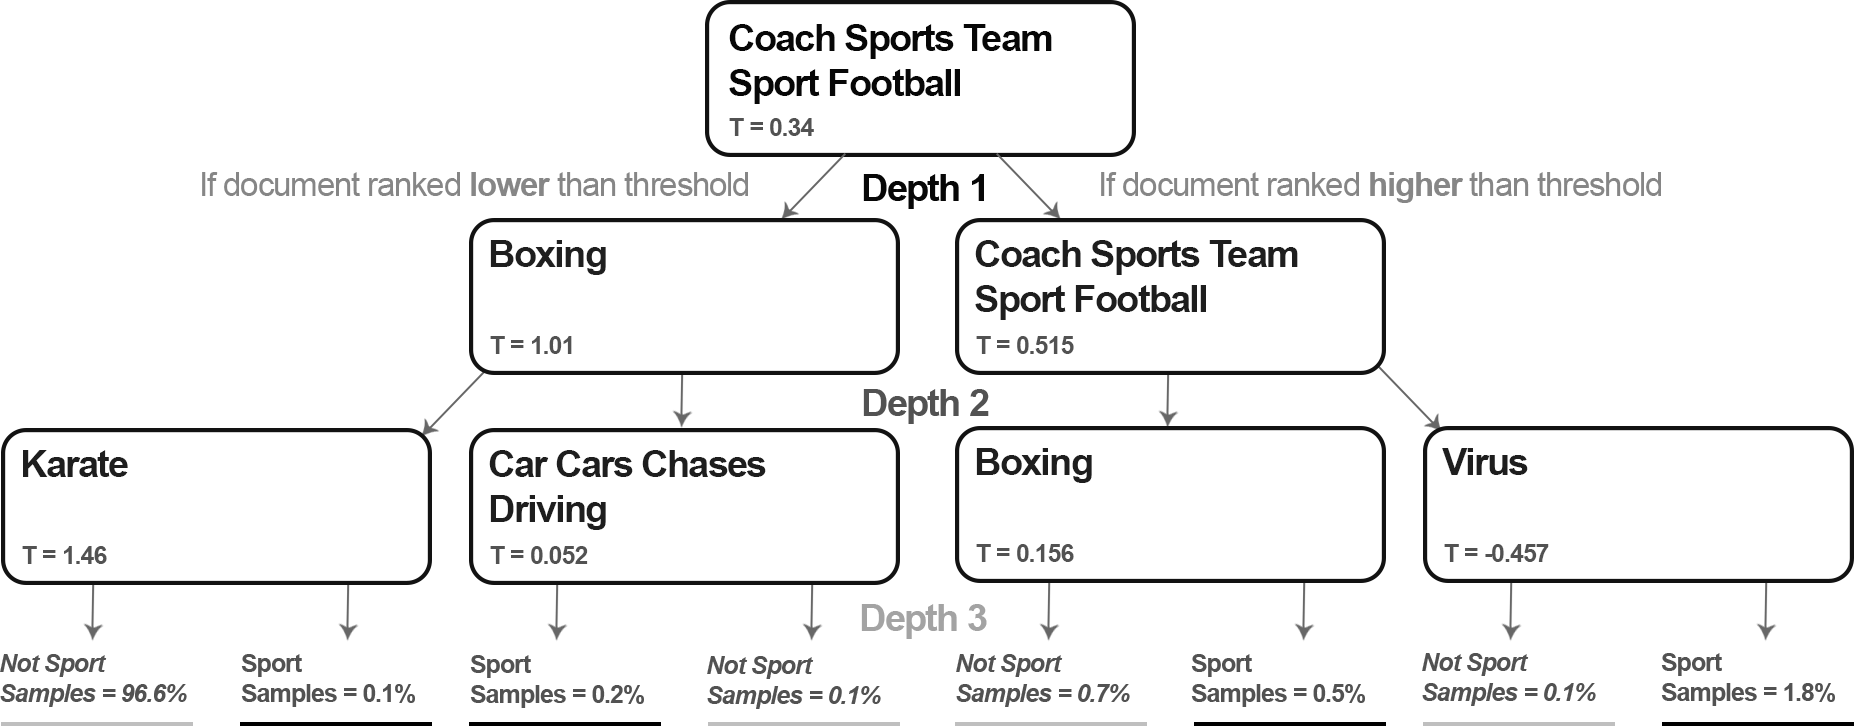
\includegraphics[width=450px]{images/decision_tree_ex.png}
	\centering
	\caption{An example of a Decision Tree classifying if a movie, represented by a concatenation of movie reviews, is in the "Sports" genre. Each Decision Tree Node corresponds to a feature, and the threshold T is the required ranking of a document on that feature to traverse right down the tree instead of left. One interesting point to note is that the most important direction is used twice, the "coach, sports, team, sport, football" cluster and results in a majority of negative samples. Another point is that the nodes at depth three are more specific, sometimes overfitting (e.g. in the case of the "Virus" node, likely overfitting to a single movie about a virus) }\label{ch1:DecisionTree}
\end{figure}

In Chapter \ref{ch4} the method described in Chapter \ref{ch3} is used to qualitatively investigate the hidden layers of neural networks, specifically feed-forward networks and auto-encoders. Feed-forward networks are trained on supervised data to classify key domain tasks, and auto-encoders are trained to find a new representation. In-order to investigate these networks, the hidden layers of the trained models are re-organized into disentangled feature representations. These disentangled feature representations are quantitatively tested using depth-3 decision trees and the predictive performance of these decision trees is compared to the neural networks. It is found that in some domains, the disentangled feature representations obtained from neural networks when used as input to decision trees match or even out-perform the neural networks they were learned from. A qualitative investigation of the disentangled features from feed-forward networks is conducted and they are found to be meaningful. Finally, auto-encoders are used to obtain a sequence of increasingly low-dimensional vector space embeddings with the understanding that each one will model more abstract concepts, and these layers are qualitatively investigated. The ability to find relationships  using the directions obtained from these layers is investigated  by attempting to build a domain theory that goes from specific features in the earlier layers to more abstract ones in the later layers. This work was published in NeSy'16, the Eleventh International Workshop on Neural-Symbolic Learning and Reasoning.

In Chapter \ref{ch5} we identify an issue with the use of the similarity centred objective used to build the vector space embedding. Specifically, although the vector spaces can be re-organized into meaningful directions, the similarity objective can sometimes be counterproductive by e.g. ranking entities that are unrelated to the feature as they are spatially an outlier. Following this, a method is introduced to fine-tune the vector space, improving the directions in the vector space embedding at the expense of modelling similarity: First, Positive Pointwise Mutual Information (PPMI) scores for the words that label the interpretable features are obtained. Then, a target ranking for each feature is found by using isotonic regression to obtain values inbetween the PPMI scores and the rankings of the entities. This target ranking is used to train a single layer neural network with a non-linear activation function that attempts to match the rankings of entities to the target ranking. The intention is not to achieve 100\% accuracy, but instead rearrange the rankings so that similarity based information is de-prioritized if it allows us to learn more meaningful directions. This results in a performance increase in some low-depth decision trees,  and a qualitatively investigation shows that the entity rankings become more specific and meaningful for the features. This work was published in The SIGNLL Conference on Computational Natural Language Learning (CoNLL) 2018.

%In particular, we use this method of building a representation of entities as a way to convert a vector space into an interpretable representation, for use in an interpretable classifier. The reason that we chose this representation to expand on is because by representing each entity $e$ with a vector $v$ that corresponds to a ranking $r$, the meaning of each dimension is distinct, and we are able to find labels composed of clusters of words for these dimensions. Here, we make the distinction between a property and a word, a property is a natural property of the space that exists in terms of a ranking of entities, and words are the labels we use to describe this property.

%%% HYPOTHESIS


% Introduction to the internet, data, basic text representations
% Introduction to machine learning, benefits of data for machine learning, machine learning representations
% Problems with machine learning, interpretability, lack of interpretability in machine learningg
% We introduce a series of methods for transforming uninterpretable machine learning representations into interpretable ones
% Finding directions in vector spaces and using those to produce interpretable representations
% Fine-tuning these directions to get a better result
% Interpreting and investigating neural networks with these directions


%This brings up an essential point: When using a semantic space, are we taking advantage of relationships that are discriminative or incorrect? The danger of relying on these spaces and the models that use them has greatly affected their adoption in critical application areas like medicine, %Citation needed
%and has raised legal concerns about their application in e.g. determining if someone is suitable for a loan. 


\section{Thesis Structure}

\begin{itemize}
	\item \textbf{Chapter \ref{ch2}} gives an overview of methods for processing unstructured text data, standard machine-learning classifiers, and it provides a background on interpretable representations.
	\item \textbf{Chapter \ref{ch2.5}} introduces and explains the datasets used in this thesis, as well as giving an introduction to the hyper-parameters  used for the machine-learning models in this thesis.
	\item \textbf{Chapter \ref{ch3}} quantitatively and qualitatively investigates how the method introduced by Derrac \cite{Derrac2015} can produce disentangled representations. In particular, we introduce the use of new scoring functions in this method, specifically NDCG, the use of standard k-means,  and comprehensively analyse the relative performance of all variants across different document representations and domains. 
	\item \textbf{Chapter \ref{ch4}} qualitatively investigates the use and application of the method in Chapter \ref{ch3} to neural networks, in particular feed-forward networks and auto-encoders.
	\item \textbf{Chapter \ref{ch5}} introduces a  method to improve the interpretable feature representation by prioritizing these features over the similarity information that is captured in the vector space.
	\item \textbf{Chapter \ref{ch6}} provides conclusions on the contributions of this thesis and outlines a number of possible avenues for future work.
\end{itemize}


\section{Summary}

This thesis experimentally validates and improves on a methodology for obtaining disentangled feature representations for text documents. It is validated using document classification tasks, and disentangled features from neural networks are  qualitatively  analysed. The method is unsupervised, acts as a post-processing step on vector space representations, and  disentangles important semantic relationships in the space.  

% Our work is...

%\section{Relationships}

%Vector spaces are representations that reduce the dimensionality of sparse representations like bag-of-words into dense spaces where semantic relationships e.g. two movies being similar to one another, are represented spatially. However, upon reducing this dimensionality the features are no longer interpretable.  One way to interpret what these vector spaces mean follows Conceptual Spaces \ref{????}, where entities in the domain e.g. movies in a domain of movie reviews are represented as points, and properties in the domain are represented as convex regions. The work in Chapter \ref{ch3} details a process where the vector space is transformed so that these properties are used as features, creating an interpretable but dense representation. The introduction goes into further detail about these properties.
% Conceptual spaces

% properties

% using properties as features

%\section{Contributions}\label{ch1:contributions}

% chapter 3 does this
%etc

%\section{Representations}




%\section{Motivation}
%What is text? How is it motivating?

%What are the desiradata of a good representation?
% Unsupervised


%One task of Natural Language Processing is to obtain this semantic understanding from text by obtaining a machine-readable representation that contains domain knowledge. A basic approach to obtain a representation of this text is to represent entities (e.g. reviews, text-posts) by the frequency of their words, see \ref{Bag-of-words-example}.

%\begin{figure}[t]
%	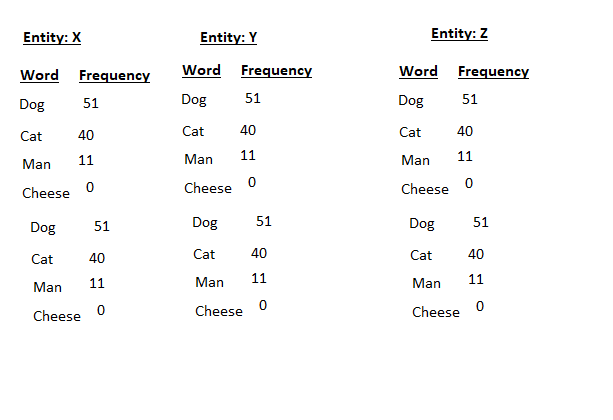
\includegraphics[width=\textwidth]{images/bowbowbow.png}
%	\centering
%	\caption{Bag-of-words  }\label{Bag-of-words-example}
%\end{figure}


 %Below, we show a review with its associated properties labelled.

%\begin{figure}[t]
%	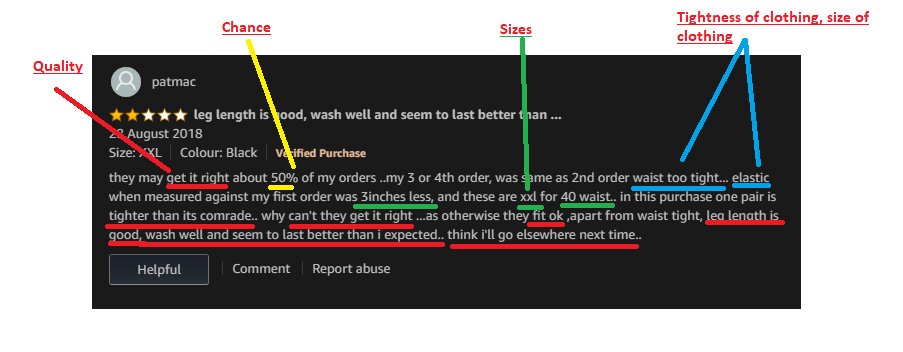
\includegraphics[width=\textwidth]{images/leg_length.png}
%	\centering
%	\caption{Example properties  }\label{IntroDecisionTree}
%\end{figure}

%\subsection{Machine Learning}
% what is machine learning? why do i care?


% Granular
%We can understand these properties to have a degree to which they apply, for example the size of the clothing might be "XXL", "XL", "L", "M" or "S", or the quality may be "Very good", "Good", "Ok", "Bad" or "Very bad". For the former, we may rely on the metadata available from the site itself, but for the latter the way to obtain this information is less clear. Although we may infer that the rating has some indication of these properties, it does not describe the properties or the degree to which the review refers to them. %This kind of information is valuable for making sense of the world of unstructured text, and has broad applications, e.g. The most immediate example is perhaps that they allow for a natural way to implement critique-based recommendation systems, where users can specify how their desired result should relate to a given set of suggestions \cite{viappiani2006preference}. For instance, \cite{Vig:2012:TGE:2362394.2362395} propose a movie recommendation system in which the user can specify that they want to see suggestions for movies that are ``similar to this one, but scarier''. If the property of being scary is adequately modelled as a direction in a semantic space of movies, such critiques can be addressed in a straightforward way. Similarly, in \cite{kovashka2012whittlesearch} a system was developed that can find ``shoes like these but shinier'', based on a semantic space representation that was derived from visual features. Semantic search systems can use such directions to interpret queries involving gradual and possibly ill-defined features, such as ``\emph{popular} holiday destinations in Europe'' \cite{DBLP:conf/sigir/JameelBS17}. While features such as popularity are typically not encoded in traditional knowledge bases, they can often be represented as semantic space directions.  %Copied from CONLL

%\subsection{Directions}\label{intro:directions}


%However, manually labelling these properties and the degrees to which entities (e.g. reviews, text-posts) have them is extremely time-consuming. 

%A potentially ideal system would be as follows: We collect large amounts of unstructured text data, separated into domains, and obtain the properties of each domain from this data, and rank entities on the degree to which they have these properties. In this way, properties would be understood on a scale built from the domain directly, so that each domain has its own meanings for words according to their own idiosyncrasies. As the process does not require any manual labelling the quality of these properties could be improved simply by obtaining more data. Further, as we are learning from unstructured data, not only would this allow us to understand the data in terms of what we know, but it would also introduce us to new ideas that we may not have previously understood. This kind of representation also has value in application to Machine Learning tasks. If we can separate the semantics of the space linearly into properties, we are able to learn simple linear classifiers that perform well. 

%Simple linear classifiers built from a representation composed of rankings on properties have an additional benefit of being more understandable.


% Natural clustering
% Semantically distinct
% Interpretable
% Curse of dimensionality
% Generalizability ("shared factors across many tasks" \cite{Bengio2012})

%What is machine learning? What are its advantages? How is it motivating?

%What are the problems with machine learning? How is it motivating?


%What is domain-specific? What is domain knowledge? %On the web there is a large volume of raw text data, e.g. Reviews of products, movies, anime, books, music, social posts by individuals, self-descriptive text about a website or product, and so on. These can be categorized into domains; each domain has its own quirks, knowledge, and method of being brought about. Although a movie review may sound similar to a book review, they typically differ hugely in the distribution of words used.

%

%\section{Interpretability}\label{ch1:interpret}

%What is interpretability? How is the value of interpretability measured in the real world?

%How can we meet the needs of the real world?  Is it transparancy, the system having easy to understnad components, etc... what  are the different views on what an interpretabile system is?

%What specific interpretability task are we trying to solve? How do we define interpretability? Why is it valuable, where is it used? What was the hypothesis/research question?
%%What are distributional models?
%Most successful approaches in recent times, like vector-spaces, word-vectors, and others, rely on the distributional model of semantics. This model relies on encoding unstructured text e.g. of a movie review, as a vector, where each dimension corresponds to how frequent each word is, we are able to calculate how similar the entities are, e.g. we know that if two movies have a similar distribution of words in their reviews, like frequent use of the word 'scary', or 'horror', then they would have a higher similarity value. These models, also known as 'semantic spaces' encode this similarity information spatially.

%Semantic relationships can be obtained from semantic spaces. 

%applications/need for good interpretability:

%What is a conceptual space? What are entities?  What are properties? What is commonsense reasoning?
%properties of an interpretable classifier:
%\begin{itemize}
%	\item Complexity: 'the magic number is seven plus or minus two' \cite{Saaty2003} also has many positive effects for its users, like lower response times \cite{Narayanan2018, Huysmans2011}, better question answering and confidence for logical problem questions \cite{Huysmans2011} and higher satisfaction \cite{Narayanan2018}.
%	\item Transparancy: 
%	\item Explainability: 
%	\item Generalizability:
%\end{itemize}


%X%X%What is a symbolic approach?  %One approach to making sense of these domains is to produce rules from expert knowledge. An expert in movies would tell you that if the review talks about it being a "cannibal horror film", we can understand that it is likely a scary movie and is related to the original 'Cannibal Holocaust' movie. Encoding this kind of knowledge is difficult, time-consuming, and hard to automate reliably.

%Properties, entities, the benefits and application of a representation formed of these

%Basic introduction to directions, explanation of the utility and application of our approach
%\section{Thesis Overview / Contributions}

%What were our objectives starting out? 
%What are our intentions with how the work in the thesis will be used?
%What are our contributions?
%%What are our aims for this chapter? What do we overall want to do? (Already kind-of said in Chapter 1, but worth repeating I guess in some form)
%In \ref{Chapter3}, we introduce a pipeline that starts with unstructured text, and ends with an interpretable representation of entities represented by properties labelled by clusters of words. Further, we demonstrate the applicability of these representations in a simple Decision Tree that uses just a few of these properties to classify entities. In Figure \ref{ExamplesWithTree}, we show some example movie entities, their associated properties, and a Decision Tree classifying whether or not they are a Horror movie. 

